%================================================================
\chapter{Hyperparameter Tables and Training Curves}
\label{app:hyperparameters}
%================================================================

\section{Full Hyperparameter Listing}
\label{app:hyperparams_table}

Table~\ref{tab:app_hyperparams} lists the hyperparameters used for
all experiments in this thesis. Where a value differs across
networks, the Modena value is listed (Net1 uses hidden dim 32
throughout because the small graph saturates at lower capacity).

\begin{table}[htbp]
  \centering
  \caption{Hyperparameters for all model variants.}
  \label{tab:app_hyperparams}
  \begin{tabular}{lll}
    \toprule
    Parameter & Value & Notes \\
    \midrule
    \multicolumn{3}{l}{\textit{Shared backbone}} \\
    GNN type          & GraphSAGE     & Best in backbone ablation \\
    Hidden dim        & 48 (32 Net1)  & \\
    GNN layers        & 2             & \\
    Dropout           & 0.1           & \\
    \midrule
    \multicolumn{3}{l}{\textit{Temporal model}} \\
    Window size $T$   & 6             & \\
    GRU hidden dim    & 48            & Same as backbone \\
    GRU layers        & 1             & \\
    Temporal features & 9             & Appended to node features \\
    \midrule
    \multicolumn{3}{l}{\textit{MoE defender}} \\
    Num experts $K$   & 6             & One per attack type + clean \\
    Router hidden     & 32            & Lighter than experts \\
    Router layers     & 2             & \\
    $\lambda_\text{anomaly}$ & 1.0  & \\
    $\lambda_\text{physics}$ & 0.1  & \\
    $\lambda_\text{router}$  & 0.5  & \\
    $\lambda_\text{balance}$ & 0.01 & \\
    \midrule
    \multicolumn{3}{l}{\textit{Self-play}} \\
    Attacker backbone & GraphSAGE 64  & \\
    Attacker MoE size & 4             & \\
    $\varepsilon_p$   & 5.0 m         & \\
    $k_p$             & 15            & \\
    $\varepsilon_q$   & 0.05 CMS      & \\
    $k_q$             & 10            & \\
    $\lambda_\text{recon}$   & 5.0  & Attacker damage weight \\
    $\lambda_\text{phys}$    & 0.05 & \\
    $\lambda_\text{div}$     & 0.5  & Attacker diversity \\
    $\lambda_\text{atk-bal}$ & 0.1  & \\
    Attacker steps $S_a$     & 3    & \\
    Defender steps $S_d$     & 1    & \\
    Curriculum threshold $\tau$ & 0.85 & \\
    Curriculum $\Delta\varepsilon$ & 0.5 m & \\
    Curriculum $\Delta k$    & 2    & \\
    \midrule
    \multicolumn{3}{l}{\textit{Training}} \\
    Optimiser         & Adam          & $\beta_1=0.9$, $\beta_2=0.999$ \\
    Learning rate     & $10^{-3}$     & \\
    Batch size        & 8             & \\
    Epochs            & 60            & \\
    Pos weight (BCE)  & 5.0           & Class-imbalance correction \\
    \bottomrule
  \end{tabular}
\end{table}

\section{Training Loss Curves}
\label{app:training_curves}

Figure~\ref{fig:app_coevolution} shows the co-evolution of attacker
and defender during the self-play loop on Modena. The defender's
adversarial F1 (navy, left axis) and the attacker loss (orange
dashed, right axis) oscillate in the expected pattern: when the
attacker improves, the defender's F1 drops; when the defender adapts,
the attacker loss rises. Dotted vertical lines mark auto-curriculum
budget increases.

\begin{figure}[htbp]
  \centering
  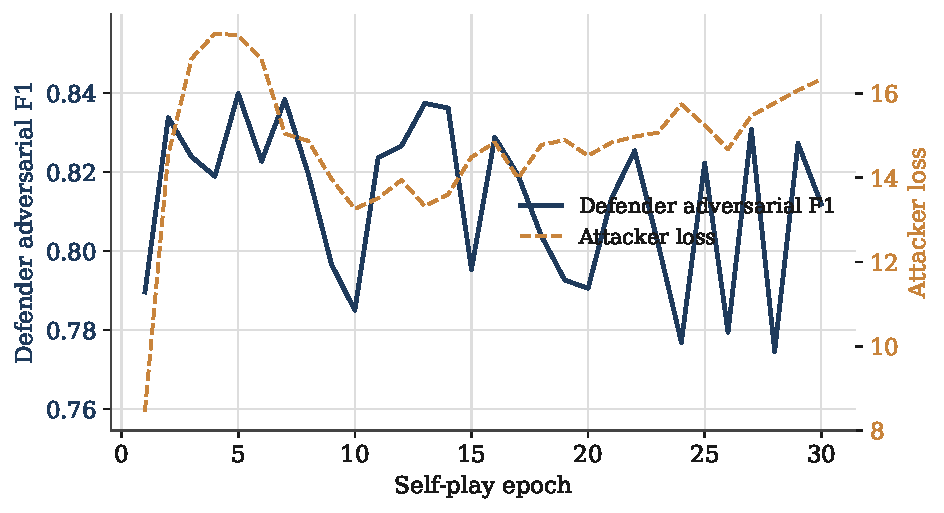
\includegraphics[width=0.9\textwidth]{figures/selfplay_coevolution}
  \caption{Attacker-defender co-evolution during self-play on Modena.
  The auto-curriculum fires three times (vertical dashed lines),
  each time the defender surpasses the 0.85 threshold.}
  \label{fig:app_coevolution}
\end{figure}

\section{Net3 Multi-Seed Results}
\label{app:net3_multiseed}

Table~\ref{tab:app_net3_multiseed} reports three-seed results for
self-play on Net3. The variance is lower than on Modena because Net3's
smaller graph (97 nodes) leaves less room for training noise.

\begin{table}[htbp]
  \centering
  \caption{Multi-seed self-play results on Net3 (three seeds).}
  \label{tab:app_net3_multiseed}
  \begin{tabular}{lrrr}
    \toprule
    Metric & Seed 1 & Seed 2 & Seed 3 \\
    \midrule
    Anomaly F1  & 0.769 & 0.761 & 0.756 \\
    P-MAE (m)   & 0.075 & 0.078 & 0.077 \\
    AUROC       & 0.941 & 0.938 & 0.937 \\
    \bottomrule
  \end{tabular}
\end{table}

\section{Dashboard Pages}
\label{app:dashboard}

The interactive Streamlit dashboard at \texttt{dashboard/app.py}
exposes all results through nine pages:

\begin{enumerate}
  \item \textbf{Network Overview} — topology viewer with per-node
    property colouring.
  \item \textbf{Reconstruction} — ground truth vs.\ observed
    vs.\ \gnn{} prediction per sensor.
  \item \textbf{Attack Analysis} — per-attack-type detection
    curves for all three networks.
  \item \textbf{Model Comparison} — architecture progression table.
  \item \textbf{Explainability} — GNNExplainer feature and
    neighbourhood importance for flagged sensors.
  \item \textbf{Self-Play} — co-evolution curves, per-attack F1,
    multi-seed box plots, held-out generalisation.
  \item \textbf{GNN Ablation} — backbone comparison bar chart.
  \item \textbf{Architecture} — diagram and parameter counts.
  \item \textbf{Live Attack} — interactive demo: inject an attack
    and watch the model flag it in real time.
\end{enumerate}
